\documentclass[12pt,utf8,notheorems,compress,t]{beamer}
\usepackage{etex}

\usepackage[english]{babel}

\usepackage{mathtools}
\usepackage{booktabs}
\usepackage{array}
\usepackage{ragged2e}
\usepackage{multicol}
\usepackage{tabto}
\usepackage{xstring}
\usepackage{mathtools}
\usepackage{soul}\setul{0.3ex}{}
\usepackage[all]{xy}
\xyoption{rotate}
\usepackage{tikz}
\usetikzlibrary{calc,shapes.callouts,shapes.arrows}

\usepackage[protrusion=true,expansion=true]{microtype}

\newcommand{\A}{\mathcal{A}}
\renewcommand{\AA}{\mathbb{A}}
\newcommand{\E}{\mathcal{E}}
\newcommand{\F}{\mathcal{F}}
\renewcommand{\G}{\mathcal{G}}
\renewcommand{\O}{\mathcal{O}}
\newcommand{\K}{\mathcal{K}}
\newcommand{\NN}{\mathbb{N}}
\newcommand{\ZZ}{\mathbb{Z}}
\newcommand{\ppp}{\mathfrak{p}}
\newcommand{\defeq}{\vcentcolon=}
\newcommand{\defeqv}{\vcentcolon\equiv}
\newcommand{\Sh}{\mathrm{Sh}}
\newcommand{\Set}{\mathrm{Set}}
\newcommand{\Sch}{\mathrm{Sch}}
\newcommand{\Hom}{\mathrm{Hom}}
\DeclareMathOperator{\Spec}{Spec}
\newcommand{\RelSpec}{\operatorname{\text{\ul{$\mathrm{Spec}$}}}}
\renewcommand{\_}{\mathpunct{.}}
\newcommand{\?}{\,{:}\,}
\newcommand{\speak}[1]{\ulcorner\text{\textnormal{#1}}\urcorner}
\newcommand{\ull}[1]{\underline{#1}}

\setlength\parskip{\medskipamount}
\setlength\parindent{0pt}

\title{Using the internal language of toposes in algebraic geometry}
\author{Ingo Blechschmidt}
\date{November 27th, 2015}

\usetheme{Warsaw}
\usecolortheme{seahorse}
%\usefonttheme{default}?
%\usepackage{kurier}?
\usefonttheme{serif}
%\usepackage{libertine}?
\usepackage{mathpazo}
\useinnertheme{rectangles}

\setbeamertemplate{blocks}[rounded][shadow=false]

\newenvironment{changemargin}[2]{%
  \begin{list}{}{%
    \setlength{\topsep}{0pt}%
    \setlength{\leftmargin}{#1}%
    \setlength{\rightmargin}{#2}%
    \setlength{\listparindent}{\parindent}%
    \setlength{\itemindent}{\parindent}%
    \setlength{\parsep}{\parskip}%
  }%
  \item[]}{\end{list}}

\newcommand{\pointthis}[2]{%
  \tikz[remember picture,baseline]{\node[anchor=base,inner sep=0,outer sep=0]%
    (#1) {#1};\node[overlay,rectangle callout,%
    callout relative pointer={(-0.2cm,0.8cm)},fill=blue!20] at ($(#1.north)+(1.8cm,-1.4cm)$) {#2};}%
}%

\newcommand{\hcancel}[5]{%
  \tikz[baseline=(tocancel.base)]{
    \node[inner sep=0pt,outer sep=0pt] (tocancel) {#1};
    \draw[red, line width=0.4mm] ($(tocancel.south west)+(#2,#3)$) -- ($(tocancel.north east)+(#4,#5)$);
  }%
}

\newcommand{\slogan}[1]{%
  \begin{center}%
    \setlength{\fboxrule}{0pt}%
    \setlength{\fboxsep}{-14pt}%
    {\usebeamercolor[fg]{item}\fbox{\usebeamercolor[fg]{normal
    text}\parbox{0.9\textwidth}{\begin{center}#1\end{center}}}}%
  \end{center}%
}

\setbeamertemplate{frametitle}[default][colsep=-2bp,rounded=false,shadow=false,center]

\setbeamertemplate{headline}{}
\setbeamertemplate{navigation symbols}{}

\newcounter{framenumberpreappendix}
\newcommand{\backupstart}{
  \setcounter{framenumberpreappendix}{\value{framenumber}}
}
\newcommand{\backupend}{
  \addtocounter{framenumberpreappendix}{-\value{framenumber}}
  \addtocounter{framenumber}{\value{framenumberpreappendix}} 
}

\setbeamertemplate{footline}{%
  \begin{beamercolorbox}[wd=\paperwidth,ht=2.5ex,dp=1.25ex,right,rightskip=1mm,leftskip=1mm]{frametitle right}
    {\quad} \inserttitle \hfill \insertauthor \quad
    \insertframenumber\,/\,\inserttotalframenumber {\quad}
  \end{beamercolorbox}}

\newcommand{\hil}[1]{{\usebeamercolor[fg]{item}{\textbf{#1}}}}

\IfSubStr{\jobname}{\detokenize{nonotes}}{
  \setbeameroption{hide notes}
}{
  \setbeameroption{show notes}
}
\setbeamertemplate{note page}[plain]

\begin{document}

\begin{frame}[c]
  \centering
  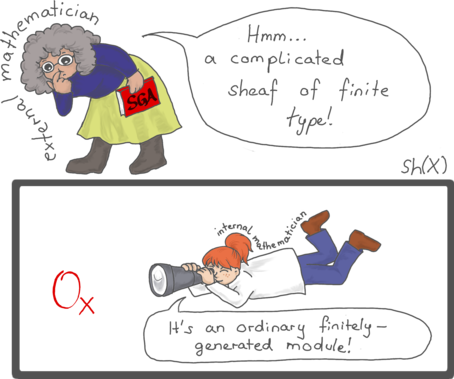
\includegraphics[scale=0.3]{images/external-internal-small}
  \medskip

  \hil{Using the internal language of toposes in \\ algebraic geometry}
  \medskip

  \scriptsize
  Ingo Blechschmidt \\
  University of Augsburg
  \medskip

  Topos à l'IHÉS \\
  November 27th, 2015
  \par
\end{frame}

\backupstart
\frame[t]{\frametitle{Outline}\scriptsize\begin{itemize}\item[]\tableofcontents\end{itemize}}

\note{\justifying\fontsize{8pt}{9.6}\selectfont
  \begin{center}\large\textbf{Abstract}\end{center}

  \begin{changemargin}{2.5em}{2.5em}
    We describe how the internal language of certain
    toposes, the associated petit and gros Zariski toposes of a scheme, can be
    used to give simpler definitions and more conceptual proofs of the basic
    notions and observations in algebraic geometry.
    % This is useful for studying schemes from a local or relative point of view.

    The starting point is that, from the internal point of view, sheaves of rings
    and sheaves of modules look just like plain rings and plain modules.
    In this way, some concepts and statements of scheme theory can be reduced to
    concepts and statements of intuitionistic linear algebra.

    Furthermore, modal operators can be used to model phrases such as ``on a
    dense open subset it holds that'' or ``on an open neighbourhood of a given
    point it holds that''. These operators define certain subtoposes; a
    generalization of the double-negation translation is useful in order to
    understand the internal universe of those subtoposes from the internal point
    of view of the ambient topos.

    A particularly interesting task is to internalize the
    construction of the relative spectrum, which, given a quasicoherent sheaf of algebras
    on a scheme~$X$, yields a scheme over~$X$. From the internal point of
    view, this construction should simply reduce to an intuitionistically sensible
    variant of the ordinary construction of the spectrum of a ring, but it turns
    out that this expectation is too naive and that a refined approach is
    necessary.
  \end{changemargin}
}

\begin{frame}[plain,c]
  \centering
  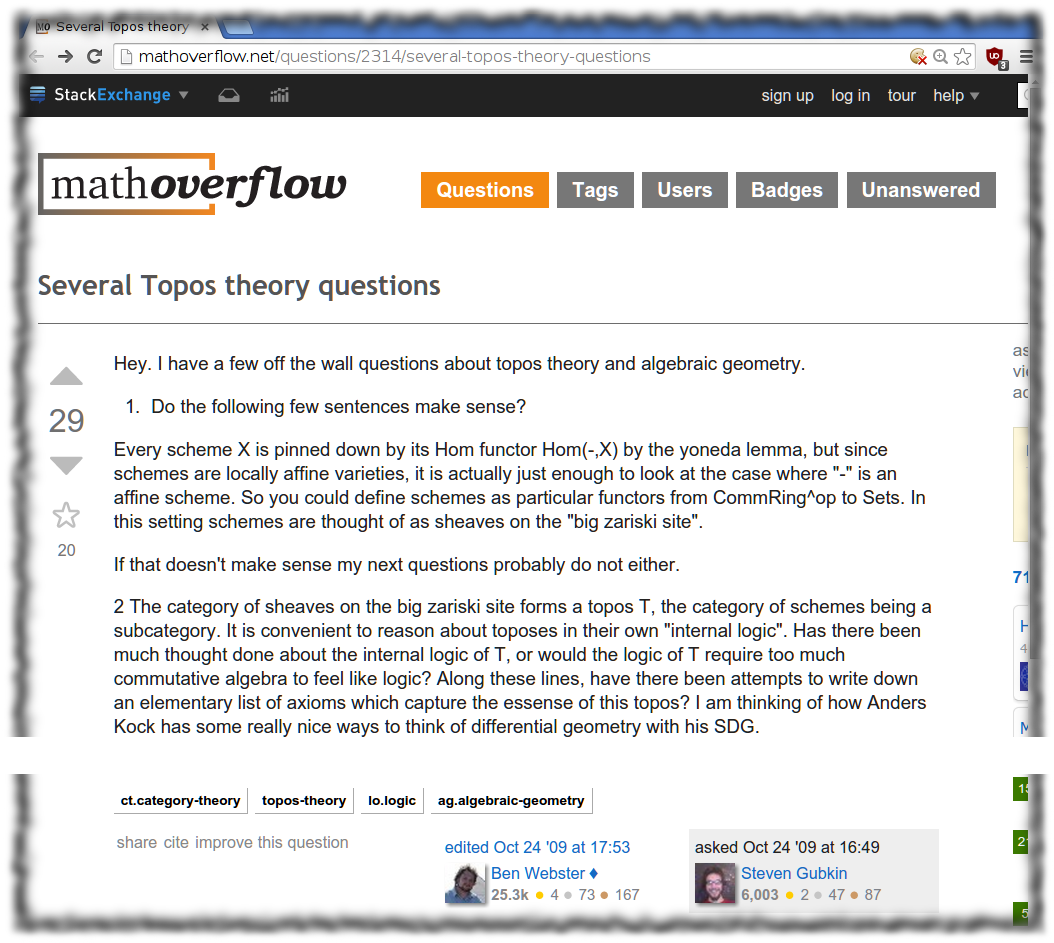
\includegraphics[scale=0.37]{images/math-overflow-steven-gubkin}
  \par
\end{frame}
\backupend


\section{Basic applications of the internal language}

\begin{frame}\frametitle{Exploiting the internal language}
  A \hil{scheme} is a locally ringed space~$(X,\O_X)$ which is
  locally isomorphic to the \hil{spectrum of a commutative ring}:
  \[ \Spec A \defeq \{ \ppp \subseteq A \,|\, \text{$\ppp$ is a prime ideal} \} \]
  \pause
  The topos~$\Sh(X)$ is the \hil{petit Zariski topos} of~$X$.

  \begin{center}
    \small
    \begin{tabular}{ll}
      \toprule
      externally & internally to $\Sh(X)$ \\
      \midrule
      sheaf of sets & set/type \\
      morphism of sheaves & map of sets \\
      monomorphism & injective map \\
      epimorphism & surjective map \\
      sheaf of rings & ring \\
      sheaf of modules & module \\
      \bottomrule
    \end{tabular}
  \end{center}
\end{frame}

\begin{frame}\frametitle{Building a dictionary}
  \slogan{\hil{Understand notions of algebraic geometry
  as notions of algebra internal to~$\boldsymbol{\Sh(X)}$.}}
  \begin{center}
    \small
    \scalebox{0.93}{\begin{tabular}{ll}
      \toprule
      externally & internally to $\Sh(X)$ \\
      \midrule
      sheaf of sets & set/type \\
      morphism of sheaves & map of sets \\
      monomorphism & injective map \\
      epimorphism & surjective map \\
      \midrule
      sheaf of rings & ring \\
      sheaf of modules & module \\
      sheaf of finite type & finitely generated module \\
      finite locally free sheaf & finite free module \\
      coherent sheaf & coherent module \\
      tensor product of sheaves & tensor product of modules \\
      rank function & minimal number of generators \\
      sheaf of rational functions & total quotient ring of~$\O_X$ \\
      \bottomrule
    \end{tabular}}
  \end{center}

  \visible<2>{\begin{tikzpicture}[overlay]
    \draw[fill=white, draw=white, opacity=0.9] (0,0) rectangle (\paperwidth,7.1);
    \node[anchor=south west,inner sep=0] (image) at (1.8,1.3) {
      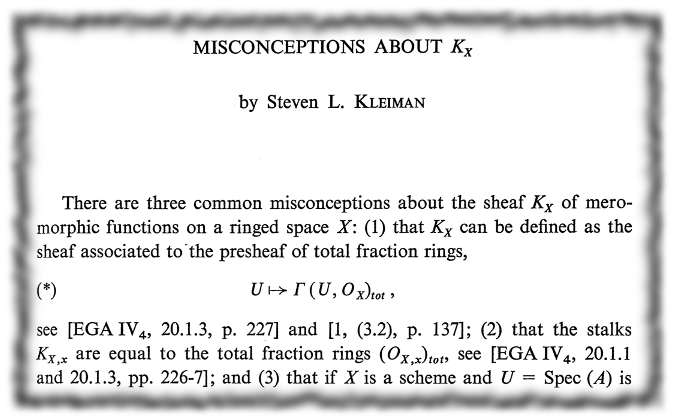
\includegraphics[width=0.7\textwidth]{images/steven-kleiman-misconceptions-about-kx}
    };
  \end{tikzpicture}}
\end{frame}

\note{\justifying
  See the \href{https://github.com/iblech/internal-methods/raw/master/notes.pdf}{notes} for more dictionary entries.

  The simple definition of~$\K_X$ allows to give an internal account of the
  basics of the theory of Cartier divisors, for instance giving an easy
  description of the line bundle associated to a Cartier divisor.
  \par
}

\begin{frame}[c]\frametitle{Praise for Mike Shulman}
  \centering
  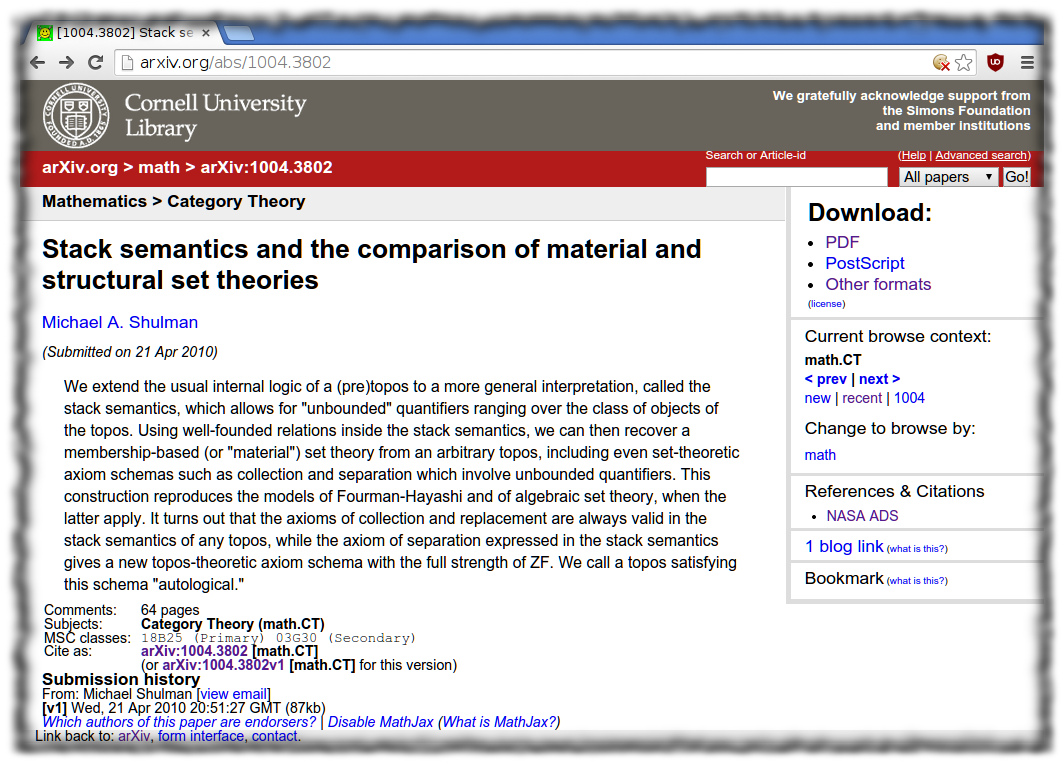
\includegraphics[scale=0.4]{images/mike-shulman-stack-semantics}
  \par
\end{frame}

\note{\justifying
  The internal language of a topos supports
  \begin{itemize}
  \item first-order logic,
  \item higher-order logic (for instance quantification over subsets),
  \item dependent types, and
  \item unbounded quantification.
  \end{itemize}

  The first three items are standard. The fourth is due to Mike Shulman.
  Combined, it's possible to interpret ``essentially all of constructive
  mathematics'' internal to a topos.

  Restrictions persist for operations with a ``set-theoretical flavor'' like
  building an infinite union of iterated powersets, for example~$\bigcup_{n \in
  \NN} P^n(\NN)$.
  \par
}

\begin{frame}\frametitle{Using the dictionary}
  \begin{center}
    \begin{minipage}{0.75\textwidth}
      \begin{exampleblock}{}
        \justifying
        Let~$0 \to M' \to M \to M'' \to 0$ be a short exact sequence of
        modules. If~$M'$ and~$M''$ are finitely generated, so is~$M$.
      \end{exampleblock}
    \end{minipage}
    \medskip

    \scalebox{3}{$\Downarrow$}

    \begin{minipage}{0.75\textwidth}
      \begin{exampleblock}{}
        \justifying
        Let $0 \to \F' \to \F \to \F'' \to 0$ be a short exact sequence
        of~$\O_X$-modules. If~$\F'$ and~$\F''$ are of finite type, so
        is~$\F$.
      \end{exampleblock}
    \end{minipage}
  \end{center}
\end{frame}

\begin{frame}[c]\frametitle{Using the dictionary}
  \begin{center}
    \begin{minipage}{0.70\textwidth}
      \begin{exampleblock}{}
        \justifying
        Any finitely generated vector space does \emph{not not} possess a basis.
      \end{exampleblock}
    \end{minipage}
    \medskip

    \scalebox{3}{$\Downarrow$}

    \begin{minipage}{0.70\textwidth}
      \begin{exampleblock}{}
        \justifying
        Any sheaf of modules of finite type on a reduced scheme is locally free
        \emph{on a dense open subset}.
      \end{exampleblock}
      \centering
      \tiny Ravi Vakil: ``Important hard exercise'' (13.7.K).
      \par
    \end{minipage}
  \end{center}
\end{frame}

\begin{frame}\frametitle{A curious property}
  Let~$X$ be a scheme. Internally to~$\Sh(X)$,
  \begin{center}
    \hil{any non-invertible element of~$\boldsymbol{\O_X}$ is nilpotent.}
  \end{center}

  \centering
  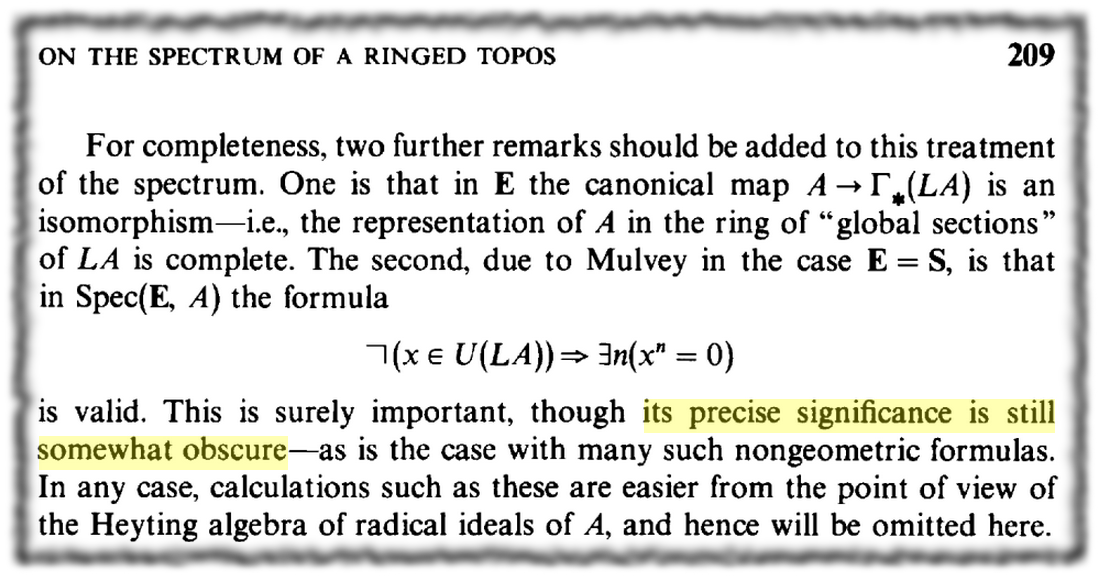
\includegraphics[scale=0.3]{images/tierney-on-the-spectrum-of-a-ringed-topos} \\
  \tiny
  %Miles Tierney. ``On the spectrum of a ringed topos''. \\ In: \emph{Algebra,
  %Topology, and Category Theory. A Collection of Papers in Honor of Samuel
  %Eilenberg}. Ed.\@ by A.~Heller and M.~Tierney. Academic Press, 1976,
  %pp.~189--210.
  Miles Tierney. On the spectrum of a ringed topos. 1976.
  \par
\end{frame}


\section{\texorpdfstring{The $\Diamond$-translation}{The ♢-translation}}

\newcommand{\idiamond}{{\usebeamercolor[fg]{item}{\boldsymbol{\Diamond}}}}
\newcommand{\gdiamond}[1]{\textcolor{gray}{\boldsymbol{\Diamond}(}#1\textcolor{gray}{)}}

\begin{frame}\frametitle{The $\Diamond$-translation}
  Let~$\E_\Diamond \hookrightarrow \E$ be a subtopos given by a \pointthis{local
  operator}{$\Diamond : \Omega_\E \to \Omega_\E$}~$\Diamond$. Then
  \[ \E_\Diamond \models \varphi \qquad\text{iff}\qquad
    \E \models \varphi^\Diamond\only<2->{.}\only<1>{,}\]
  \only<1>{where the translation~$\varphi \mapsto \varphi^\Diamond$ is given by:
  \begin{align*}
    (s = t)^\Diamond &\defeqv \idiamond(s=t) \\
    (\varphi \wedge \psi)^\Diamond &\defeqv \gdiamond{\varphi^\Diamond \wedge \psi^\Diamond} \\
    (\varphi \vee \psi)^\Diamond &\defeqv \idiamond(\varphi^\Diamond \vee \psi^\Diamond) \\
    (\varphi \Rightarrow \psi)^\Diamond &\defeqv \gdiamond{\varphi^\Diamond \Rightarrow \psi^\Diamond} \\
    (\forall x\?X\_ \varphi(x))^\Diamond &\defeqv \gdiamond{\forall x\?X\_ \varphi^\Diamond(x)} \\
    (\exists x\?X\_ \varphi(x))^\Diamond &\defeqv \idiamond(\exists x\?X\_ \varphi^\Diamond(x))
  \end{align*}}

  \only<2->{
    Let~$X$ be a scheme. Depending on~$\Diamond$,~$\Sh(X)
    \models \Diamond\varphi$ means that~$\varphi$ holds on \ldots
    \begin{itemize}
      \item \ldots{} a dense open subset.
      \item \ldots{} a schematically dense open subset.
      \item \ldots{} a given open subset~$U$.
      \item \ldots{} an open subset containing a given closed subset~$A$.
      \item \ldots{} an open neighbourhood of a given point~$x \in X$.
    \end{itemize}

    \pause
    Can tackle the question~``$\varphi^\Diamond \stackrel{?}{\Rightarrow} \Diamond\varphi$'' logically.
  }
\end{frame}

\note{\justifying
  The~$\Diamond$-translation is a generalization of the \emph{double negation
  translation}, which is well-known in logic. The double negation translation
  has the following curious property: A formula~$\varphi$ admits a classical
  proof if and only if the translated formula~$\varphi^{\neg\neg}$ admits an
  intuitionistic proof.

  The~$\Diamond$-translation has been studied before (see for instance Aczel:
  \emph{The Russell--Prawitz modality}, and Escardó, Oliva: \emph{The Peirce
  translation and the double negation shift}), but to the best of my know\-ledge,
  this application -- expressing the internal language of
  subtoposes in the internal language of the ambient topos -- is new.
  \par
}

\note{\justifying
  For ease of exposition, assume that~$X$ is irreducible with generic
  point~$\xi$. Let~$\Diamond \defeqv \neg\neg$.

  Then~$\Sh(X) \models \Diamond \varphi$ means that~$\varphi$ holds on a dense
  open subset of~$X$, while~$\Sh(X) \models \varphi^\Diamond$ means
  that~$\varphi$ holds at the generic point (taking stalks of all involved
  sheaves).

  The question~``does~$\varphi^\Diamond$ imply~$\Diamond\varphi$?'' therefore
  means: Does~$\varphi$ spread from the generic point to a dense open subset?

  For the special case of the double negation translation, a general answer to
  this purely logical question has long been known: This holds if~$\varphi$ is
  a \emph{geometric formula} (doesn't contain~$\Rightarrow$ and~$\forall$).
  \par
}

\note{\justifying
  Let~$\F$ be a sheaf of modules on a locally ringed space~$X$.
  Assume that the stalk~$\F_x$ at some point~$x \in X$ vanishes.
  Then in general it does \emph{not} follow that~$\F$ vanishes on some open
  neighbourhood of~$x$.

  This can be understood in logical terms: The statement that~$\F$ vanishes,
  \[ \forall s : \F\_\ s = 0, \]
  is not a geometric formula.

  However, if~$\F$ is additionally supposed to be of finite type, then it
  \emph{does} follow that~$\F$ vanishes on an open neighbourhood. This too can
  be understood in logical terms: If~$\F$ is of finite type, then internally
  there are generators~$s_1,\ldots,s_n$ of~$\F$. Thus the vanishing of~$\F$ can
  be reformulated as
  \[ s_1 = 0 \wedge \cdots \wedge s_n = 0, \]
  and this condition is manifestly geometric.
  \par
}


\section{Quasicoherence of sheaves of modules}

\begin{frame}\frametitle{Quasicoherence}
  Let~$X$ be a scheme. Let~$\E$ be an~$\O_X$-module.

  Then~$\E$ is quasicoherent
  if and only if, internally to~$\Sh(X)$,
  \begin{quote}\textnormal{$\E[f^{-1}]$ is a $\Diamond_f$-sheaf for any~$f : \O_X$, \\[0.3em]
  \qquad\qquad where~$\Diamond_f\varphi \defeqv (\text{$f$ invertible} \Rightarrow \varphi)$.}
  \end{quote}
  \pause

  In particular: If~$\E$ is quasicoherent, then internally
  \[ (\text{$f$ invertible} \Rightarrow s = 0) \Longrightarrow
    \bigvee_{n \geq 0} f^n s = 0 \]
  \vspace*{-1.5em}\par%
  for any~$f : \O_X$ and~$s : \E$.
\end{frame}

\note{\justifying
  The sheaf condition and the sheafification functor can be described purely
  internally. An object~$M$ is \emph{separated} with respect to~$\Diamond$ if
  and only if, from the internal point of view,
  \[ \forall x,y : M\_\ \Diamond(x = y) \Rightarrow x = y. \]
  It is a \emph{sheaf} with respect to~$\Diamond$, if furthermore
  \[ \forall K \subseteq M\_\
    \Diamond(\exists x : M\_\ K = \{ x \}) \Longrightarrow
    \exists x : M\_\ \Diamond(x \in K). \]

  The second condition displayed on the previous slide is equivalent to the
  separatedness condition. In the special case~$\E = \O_X$, $s = 1$ it reduces
  to Mulvey's ``somewhat obscure formula''. We now understand this condition in
  its proper context.
  \par
}


\section{The relative and internal spectrum}

\begin{frame}\frametitle{The absolute spectrum}
  Let~$A$ be a commutative ring (in~$\Set$).

  Is there a \hil{free local ring}~$A \to A'$ over~$A$?
  \[ \xymatrix{
    A \ar[rd] \ar[rrr] &&& {\substack{\text{local}\\\text{\normalsize$R$}\\\phantom{\text{local}}}} \\
    & {\substack{\text{\normalsize$A'$}\\\text{local}}} \ar@{-->}_[@!34]{\text{local}}[rru]
  } \]

  \hil{No,} if we restrict to~$\Set$.

  \hil{Yes,} if we allow a change of topos:
  Then $A \to \O_{\Spec A}$ is the universal localization.
\end{frame}

\note{\justifying
  Details on this point of view can be found in one of Peter Arndt's very nice
  answers on MathOverflow:
  \begin{center}\url{http://mathoverflow.net/a/14334/31233}\end{center}
  \par
}

\newcommand{\defspeca}{\text{topological space of the prime ideals of $A$}}
\newcommand{\defspecb}{\text{topological space of the prime filters of $A$}}
\newcommand{\defspecc}{\text{locale of the prime filters of $A$}}

\begin{frame}\frametitle{The absolute spectrum, internalized}
  Let~$A$ be a commutative ring in a topos~$\E$.

  To construct the \hil{free local ring} over~$A$, give a constructive account
  of the spectrum:
  \begin{align*}
    \only<1>{\Spec A &\defeq \defspeca}
    \only<2->{\Spec A &\defeq \hcancel{$\defspeca$}{0pt}{3pt}{0pt}{-2pt}}
    \\
    \only<3>{&\defeq \defspecb}
    \only<4->{&\defeq \hcancel{$\defspecb$}{0pt}{3pt}{0pt}{-2pt}}
    \\
    \only<5->{&\defeq \defspecc}
  \end{align*}
  \pause
  \pause
  \pause
  \pause
  Define the frame of opens of~$\Spec A$ to be the frame of radical ideals
  in~$A$.
  \pause

  This gives an internal description of
  Monique Hakim's spectrum functor~$\mathrm{RT} \to \mathrm{LRT}$.
\end{frame}

\note{\justifying
  Monique Hakim constructed in her thesis a very general spectrum functor,
  taking a ringed topos to a locally ringed one, using explicit calculations
  with sites.

  Using the internal language allows to reduce these calculations to a minimum.
  One constructs the spectrum as the sheaf topos over an internal
  locale and then uses the general theorem that toposes over the base~$\E$ are
  the same as toposes internal to~$\E$.

  As a byproduct one obtains that Hakim's spectrum is \emph{localic} over the base.
  \par
}

\begin{frame}\frametitle{The relative spectrum}
  Let~$X$ be a scheme and~$\O_X \xrightarrow{\varphi} \A$ be a quasicoherent algebra.
  Can we describe~\hil{$\boldsymbol{\RelSpec_X \A}$}, a scheme over~$X$, internally?

  Desired universal property:
  \[ \Hom_{\Sch/X}(T, \RelSpec_X \A) \cong \Hom_{\mathrm{Alg}(\O_X)}(\A,
  \mu_*\O_T) \]
  for all~$X$-schemes~$T \xrightarrow{\mu} X$.
  \pause

  \hil{Solution:} Define internally the frame of~$\RelSpec_X \A$ to be the frame of
  those radical ideals~$I \subseteq \A$ such that
  \[ \forall f\?\O_X\_ \forall s\?\A\_
    (\text{$f$ invertible in~$\O_X$} \Rightarrow s \in I) \Longrightarrow
      fs \in I. \]
  \pause
  Its \hil{points} are those prime filters~$G$ of~$\A$ such that
  \[ \forall f\?\O_X\_ \varphi(f) \in G \Longrightarrow \text{$f$ invertible in~$\O_X$}. \]
\end{frame}

\note{\justifying
  The stated condition on~$I$ is, under the assumption that~$\A$ is
  quasicoherent, equivalent to the condition that~$I$ is quasicoherent (as
  an~$\O_X$-module).

  The relative spectrum is thus constructed as a certain sublocale of the
  absolute one. The two constructions coincide if and only if the dimension of
  the base scheme is~$\leq 0$.

  If~$X$ is not a scheme or~$\A$ is not quasicoherent, the construction still
  gives rise to a locally ringed locale over~$X$ which satisfies the universal
  property
  \[ \Hom_{\mathrm{LRL}/X}(T, \RelSpec_X \A) \cong \Hom_{\mathrm{Alg}(\O_X)}(\A,
  \mu_*\O_T) \]
  for all locally ringed locales~$T \xrightarrow{\mu} X$ over~$X$.
  \par
}

\begin{frame}\frametitle{The relative spectrum, reformulated}
  Let~$B \to A$ be an algebra in topos.

  Is there a \hil{free local and local-over-$\boldsymbol{B}$ ring}~$A \to A'$ over~$A$?

  \[ \xymatrix{
    B \ar[r]\ar@/^2pc/[rrrr]^{\text{local}}\ar@/_/[rrd]_[@!-33]{\text{local}} &
      A \ar[rd] \ar[rrr] &&&
      {\substack{\text{local}\\\text{\normalsize$R$}\\\phantom{\text{local}}}} \\
    && {\substack{\text{\normalsize$A'$}\\\text{local}}} \ar@{-->}[rru]_[@!35]{\text{local}}
  } \]

  \medskip
  Form limits in the category of \hil{locally ringed locales}
  by \hil{relocalizing} the corresponding limit in ringed locales.
\end{frame}

\note{\justifying
  One might wonder whether the absolute spectrum or the relative one is ``more
  fundamental''. The absolute spectrum can be expressed using the relative one,
  since
  \[ \Spec A = \RelSpec_{\Spec \ZZ} A^{\sim}, \]
  but the other way is not in general possible: The absolute spectrum is always
  (quasi-)compact, while the relative one is not in general.
  \par
}
% XXX: Give details.

\backupstart

\begin{frame}
  \slogan{\hil{Understand notions and statements of algebraic geometry
  as notions and statements of algebra internal to appropriate toposes.}}

  {\vspace{-0.1em}\centering
  \rotatebox{90}{\tiny\scalebox{0.5}{Illustration: Carina Willbold}}\hspace{-0.05cm}%
  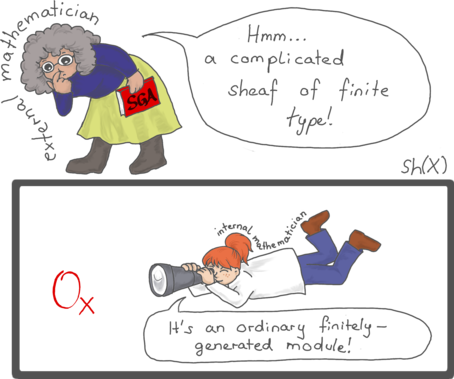
\includegraphics[scale=0.20]{images/external-internal-small}
  \par\medskip\vspace{-0.1em}}

  \begin{itemize}
    \item Simplify proofs and gain conceptual understanding.
    \item Understand relative geometry as absolute geometry.
    \item Develop a synthetic account of scheme theory.
    \item Contribute to constructive algebra.
  \end{itemize}

  \centering
  \hil{\href{http://tiny.cc/topos-notes}{http://tiny.cc/topos-notes}} \\
  \begin{minipage}{1.0\textwidth}\justifying
    \scriptsize
    spreading of properties,
    general transfer principles,
    applications to constructive algebra,
    quasicoherence,
    internal Cartier divisors,
    pullback along immersions $=$ internal sheafification,
    scheme dimension $=$ internal Krull dimension of~$\O_X$,
    dense $=$ not not,
    modal operators,
    relative spectrum,
    other toposes,
    étale topology,
    group schemes $=$ groups,
    \ldots
  \end{minipage}
  \par
\end{frame}
% Fun fact:
% Very naive definition of P^n works internal to the big Zariski topos.

\begin{frame}[plain,c]
  \centering
  
\includegraphics[scale=0.5]{images/sheafification-man}
  \sffamily

  You should totally look up:

  \hil{The Adventures of Sheafification Man}
  \par
\end{frame}


\appendix

\section{Spreading from points to neighbourhoods}

\begin{frame}\frametitle{Spreading from points to neighbourhoods}
  All of the following lemmas have a short, sometimes trivial proof.
  Let~$\F$ be a sheaf of finite type on a ringed space~$X$.
  Let~$x \in X$. Let~$A \subseteq X$ be a closed subset. Then:
  \small
  \begin{enumerate}
    \item $\F_x = 0$ iff~$\F|_U = 0$ for some open neighbourhood of~$x$.
    \item $\F|_A = 0$ iff~$\F|_U = 0$ for some open set containing~$A$.
    \item $\F_x$ can be generated by~$n$ elements iff this is true on some open
    neighbourhood of~$x$.
%   \item $\alpha_x$ is surjective iff~$\alpha$ is an epimorphism on some open
%   set containing~$x$, where~$\alpha : \G \to \F$ is any morphism.
    \item $\mathcal{H}\mathrm{om}_{\O_X}(\F,\G)_x \cong
    \Hom_{\O_{X,x}}(\F_x,\G_x)$ if~$\F$ is of finite presentation around~$x$.
    \item $\F$ is torsion iff~$\F_\xi$ vanishes (assume~$X$ integral and~$\F$ quasicoherent).
    \item $\F$ is torsion iff~$\F|_{\mathrm{Ass}(\O_X)}$ vanishes (assume~$X$
    locally Noetherian and~$\F$ quasicoherent).
  \end{enumerate}
\end{frame}

\note{\justifying
  Statements 1 and 2 follow from \emph{one} proof in the internal language,
  applied to two different modal operators.

  Similarly with statements~5 and~6.
  \par
}


\section{The meromorphic functions revisited}

\begin{frame}\frametitle{The smallest dense sublocale}
  Let~$X$ be a reduced scheme satisfying a technical condition.
  Let~$i : X_{\neg\neg} \to X$ be the inclusion of the smallest dense sublocale
  of~$X$.

  Then~$i_* i^{-1} \O_X \cong \K_X$.

  \begin{itemize}
    \item This is a highbrow way of saying ``rational functions are regular
    functions which are defined on a dense open subset''.
    \item Another reformulation is that~$\K_X$ is the sheafification of~$\O_X$
    with respect to the~$\neg\neg$-modality.
    \item There is a generalization to nonreduced schemes.
  \end{itemize}
\end{frame}


\section{Transfer principles}

\begin{frame}\frametitle{Transfer principles}
  Let~$M$ be an~$A$-module. How do~$M$ and the sheaf~$M^{\sim}$ on~$\Spec A$
  relate?

  Observe that $M^{\sim} \cong \underline{M}[\F^{-1}]$ is the localization of~$M$ at
  the \hil{generic prime filter} and that~$M$ shares all first-order properties
  with the constant sheaf of modules~$\underline{M}$. Therefore:
  \begin{center}
    $M^{\sim}$ inherits all those properties of~$M$ which are \\
    \hil{stable under localization}.
  \end{center}
  Examples: finitely generated, free, flat, \ldots

  A converse holds as well, suitably formulated.
\end{frame}


\section{Applications in algebra}

\begin{frame}\frametitle{Applications in algebra}
  Let~$A$ be a commutative ring.
  The internal language of~$\Sh(\Spec A)$ allows you to say ``without loss of
  generality, we may assume that~$A$ is local'', even constructively.

  \begin{center}
    \begin{minipage}{0.75\textwidth}
      \begin{exampleblock}{}
        \justifying
        The kernel of any matrix over a principial ideal domain is finitely
        generated.
      \end{exampleblock}
    \end{minipage}
    \medskip

    \scalebox{3}{$\Downarrow$}

    \begin{minipage}{0.75\textwidth}
      \begin{exampleblock}{}
        \justifying
        The kernel of any matrix over a Prüfer domain is finitely generated.
      \end{exampleblock}
    \end{minipage}
  \end{center}
\end{frame}

\begin{frame}\frametitle{Hilbert's program in algebra}
  \scriptsize\justifying
  There is a way to combine some of the powerful tools of classical ring theory
  with the advantages that constructive reasoning provides, for instance
  exhibiting explicit witnesses. Namely we can devise
  a language in which we can usefully talk about prime ideals, but which
  substitutes non-constructive arguments by constructive arguments ``behind
  the scenes''. The key idea is to substitute the phrase ``for all prime ideals''
  (or equivalently ``for all prime filters'') by ``for the generic prime filter''.

  More specifically, simply interpret a given proof using prime filters
  in~$\Sh(\Spec A)$ and let it refer to~$\F \hookrightarrow \underline{A}$.

  \hspace*{-0.75cm}%
  \begin{tabular}{lll}
    \toprule
    Statement & constructive substitution & meaning \\\midrule
    $x \in \ppp$ for all~$\ppp$. &
    $x \not\in \F$. &
    $x$ is nilpotent. \\
    $x \in \ppp$ for all~$\ppp$ such that~$y \in \ppp$. &
    $x \in \F \Rightarrow y \in \F$. &
    $x \in \sqrt{(y)}$. \\
    $x$ is regular in all stalks~$A_\ppp$. &
    $x$ is regular in~$\ull{A}[\F^{-1}]$. &
    $x$ is regular in~$A$. \\
    The stalks~$A_\ppp$ are reduced. &
    $\ull{A}[\F^{-1}]$ is reduced. &
    $A$ is reduced. \\
    The stalks~$M_\ppp$ vanish. &
    $\ull{M}[\F^{-1}] = 0$. &
    $M = 0$. \\
%   The stalks~$M_\ppp$ are fin.\@ gen.\@ over~$A_\ppp$. &
%   $\ull{M}[\F^{-1}]$ is fin.\@ gen.\@ over
%   $\ull{A}[\F^{-1}]$. &
%   $M$ is fin.\@ gen.\@ over~$A$. \\
    The stalks~$M_\ppp$ are flat over~$A_\ppp$. &
    $\ull{M}[\F^{-1}]$ is flat over~$\ull{A}[\F^{-1}]$. &
    $M$ is flat over~$A$. \\
    The maps~$M_\ppp \to N_\ppp$ are injective. &
    $\ull{M}[\F^{-1}] \to \ull{N}[\F^{-1}]$ is injective. &
    $M \to N$ is injective. \\
    The maps~$M_\ppp \to N_\ppp$ are surjective. &
    $\ull{M}[\F^{-1}] \to \ull{N}[\F^{-1}]$ is surjective. &
    $M \to N$ is surjective. \\
    \bottomrule
  \end{tabular}

  This is related (in a few cases equivalent) to the \emph{dynamical methods in
  algebra} explored by Coquand, Coste, Lombardi, Roy, and others. Their
  approach applies more generally.
  \par
\end{frame}


\section{The gros Zariski topos}

\begin{frame}\frametitle{The gros Zariski topos}
  Let~$X$ be a scheme. The \hil{gros Zariski topos} is the topos of sheaves
  on~$\Sch/X$ with respect to the Zariski topology. From its point of view,
  \ldots

  \begin{itemize}
    \item \ldots{} $X$-schemes look just like sets,
    \item \ldots{} $\mathbb{P}^n_X$ is given by the naive expression
    \[ \{ (x_0,\ldots,x_n) \,|\, x_1 \neq 0 \vee \cdots \vee x_n \neq 0
    \}/\text{(rescaling)}, \]
    \item \ldots{} the cotangent ``bundle'' of an~$X$-scheme~$T$ is
    \[ \text{the set of maps $\Delta \to \ull{T}$,} \]
    where~$\Delta = \{ \varepsilon \in \ull{\AA}^1_X \,|\, \varepsilon^2 = 0
    \}$.
    \item \ldots{} affinity is a ``double dual condition'', and
    \item \ldots{} the étale topology is the coarsest topology~$\Diamond$ s.\,th.
    \[ \forall f : \ull{\AA}^1_X[T]\_\
      \text{$f$ is monic separable} \Rightarrow
      \Diamond(\exists t : \ull{\AA}^1\_ f(t) = 0). \]
  \end{itemize}
\end{frame}

\note{
  \begin{itemize}\justifying
    \item The functor of points of~$\AA^1_X$, that is
    \[ \ull{\AA}^1_X : (T/X) \longmapsto \O_T(T), \]
    looks like a local ring and indeed like a field from the internal point of
    view, in the sense that
    \[ \forall f\?\ull{\AA}^1_X\_ \neg(f = 0) \Rightarrow \text{$f$
    invertible}. \]
    \item Let~$\A$ be a quasicoherent~$\O_X$-algebra. Let~$\E$ be the
    induced~$\ull{\AA}^1_X$-algebra given by~$\E(T \xrightarrow{\mu} X) \defeq
    (\mu^* \A)(T)$. Then the internal Hom set~$[\E,
    \ull{\AA}^1_X]_{\ull{\AA}^1_X}$ of~$\ull{\AA}^1_X$-algebra morphisms is the
    functor of points of~$\RelSpec_X(\A)$.
    \item Let~$\mu : T \to X$ be quasicompact and quasiseparated.
    Then~$\mu$ is affine iff, from the internal point of view, the map
    \[ \ull{T} \longrightarrow [ [\ull{T},\ull{\AA}^1_X]^\flat, \ull{\AA}^1_X ]_{\ull{\AA}^1_X},\ x \longmapsto
    \ull{\ \ }(x) \]
    into the ``double dual'' is bijective.
  \end{itemize}
}

\note{
  \begin{itemize}\justifying
    \item Describing the functor of points of the projective space was
    suggested by Zhen Lin Low.
    \item The statement on the étale topology follows from Gavin Wraith's
    article \emph{Generic Galois theory of local rings}.
  \end{itemize}
}


\section{Basics about the internal language}

\begin{frame}\frametitle{The internal language of a topos}
  Let~$\E$ be a topos. Then we can define the meaning of
  \[ \hil{$\E \models \varphi \qquad\textnormal{(``$\varphi$ holds in $\E$'')}$} \]
  for formulas~$\varphi$ over~$\E$ using the \hil{Kripke--Joyal semantics}.

  \begin{center}
    \small
    \begin{tabular}{ll}
      \toprule
      externally & internally \\
      \midrule
      object & set/type \\
      morphism & map of sets \\
      monomorphism & injective map \\
      epimorphism & surjective map \\
      \bottomrule
    \end{tabular}
  \end{center}
  \pause

  \mbox{If~$\varphi$ implies~$\psi$ \hil{intuitionistically}, then~$\E \models \varphi$
  implies~$\E \models \psi$.}
\end{frame}

\note{\justifying
  More generally, for an object~$U$ of a topos~$\E$, we define the meaning of
  \[ U \models \varphi \qquad\text{($\varphi$ holds on~$U$)}. \]
  Writing~``$\E \models \varphi$'' is then an abbreviation for~``$1 \models
  \varphi$'', where~``$1$'' denotes the terminal object of~$\E$.

  In addition to soundness with respect to intuitionistic logic, the internal
  language has the following two important properties:
  \begin{itemize}
    \item \hil{Monotonicity:} If~$p : V \to U$ is an arbitrary morphism and~$U
    \models \varphi$, then also~$V \models \varphi$.
    \item \hil{Locality:} If~$p : V \to U$ is an epimorphism and~$V \models
    \varphi$, then also~$U \models \varphi$.
  \end{itemize}
}

\note{\justifying
  In the special case that~$\E = \Sh(X)$ is the topos of sheaves on a
  topological space (or locale)~$X$, the rules of the Kripke--Joyal semantics
  look as follows. We tersely write~``$U \models \varphi$'' instead
  of~``$\Hom(\ull{\ \ }, U) \models \varphi$ for open subsets~$U \subseteq X$.
  \scriptsize
  \newcommand{\Ll}{:\Longleftrightarrow}
  \[ \renewcommand{\arraystretch}{1.3}\begin{array}{@{}lcl@{}}
    U \models f = g \? \F &\Ll& f|_U = g|_U \in \F(U) \\
    U \models \varphi \wedge \psi &\Ll&
      \text{$U \models \varphi$ and $U \models \psi$} \\
    U \models \varphi \vee \psi &\Ll&
      \hcancel{\text{$U \models \varphi$ or $U \models \psi$}}{0pt}{3pt}{0pt}{-2pt} \\
    && \text{there exists a covering $U = \bigcup_i U_i$ s.\,th. for all~$i$:} \\
    && \quad\quad \text{$U_i \models \varphi$ or $U_i \models \psi$} \\
    U \models \varphi \Rightarrow \psi &\Ll&
      \text{for all open~$V \subseteq U$: }
    \text{$V \models \varphi$ implies $V \models \psi$} \\
    U \models \forall f \? \F\_ \varphi(f) &\Ll&
      \text{for all sections~$f \in \F(V), V \subseteq U$: $V \models
      \varphi(f)$} \\
    U \models \exists f \? \F\_ \varphi(f) &\Ll&
      \text{there exists a covering $U = \bigcup_i U_i$ s.\,th. for all~$i$:} \\
    && \quad\quad \text{there exists~$f_i \in \F(U_i)$ s.\,th.
    $U_i \models \varphi(f_i)$}
  \end{array} \]
}

\begin{frame}\frametitle{Translating internal statements I}
  Let~$X$ be a topological space (or locale) and let~$\alpha : \F \to \G$ be a
  morphism of sheaves on~$X$. Then:
  \allowdisplaybreaks
  \begin{align*}
    & \Sh(X) \models \speak{$\alpha$ is injective} \\[0.5em]
    \Longleftrightarrow\
    & \Sh(X) \models \forall s\?\F\_ \forall t\?\F\_ \alpha(s) = \alpha(t) \Rightarrow s = t \\[0.5em]
    \Longleftrightarrow\ &
      \text{for all open~$U \subseteq X$, sections $s \in \F(U)$:} \\
    &\qquad
      \text{for all open~$V \subseteq U$, sections $t \in \F(V)$:} \\
    &\qquad\qquad
        \text{for all open~$W \subseteq V$:} \\
    &\qquad\qquad\qquad
          \text{$\alpha_W(s|_W) = \alpha_W(t|_W)$ implies $s|_W = t|_W$} \\[0.5em]
    \Longleftrightarrow\ &
      \text{for all open~$U \subseteq X$, sections $s, t \in \F(U)$:} \\
    &\qquad
          \text{$\alpha_U(s|_U) = \alpha_U(t|_U)$ implies $s|_U = t|_U$} \\[0.5em]
    \Longleftrightarrow\ &
      \text{$\alpha$ is a monomorphism of sheaves}
  \end{align*}
\end{frame}

\begin{frame}\frametitle{Translating internal statements II}
  Let~$X$ be a topological space (or locale) and let~$\alpha : \F \to \G$ be a
  morphism of sheaves on~$X$. Then:
  \allowdisplaybreaks
  \begin{align*}
    & \Sh(X) \models \speak{$\alpha$ is surjective} \\[0.5em]
    \Longleftrightarrow\
    & \Sh(X) \models \forall t\?\G\_ \exists s\?\F\_ \alpha(s) = t \\[0.5em]
    \Longleftrightarrow\ &
      \text{for all open~$U \subseteq X$, sections $t \in \G(U)$:} \\
    &\qquad
      \text{there exists an open covering~$U = \textstyle\bigcup_i U_i$ and} \\
    &\qquad
      \text{sections~$s_i \in \F(U_i)$ such that:} \\
    &\qquad\qquad
        \alpha|_{U_i}(s_i) = t|_{U_i} \\[0.5em]
    \Longleftrightarrow\ &
      \text{$\alpha$ is an epimorphism of sheaves}
  \end{align*}
\end{frame}

\begin{frame}\frametitle{Translating internal statements III}
  Let~$X$ be a topological space (or locale) and let~$s, t \in \F(X)$ be global
  sections of a sheaf~$\F$ on~$X$. Then:
  \allowdisplaybreaks
  \begin{align*}
    & \Sh(X) \models \neg\neg(s = t) \\[0.5em]
    \Longleftrightarrow\
    & \Sh(X) \models ((s = t) \Rightarrow \bot) \Rightarrow \bot \\[0.5em]
    \Longleftrightarrow\ &
      \text{for all open~$U \subseteq X$ such that} \\
    &\qquad
      \text{for all open~$V \subseteq U$ such that} \\
    &\qquad\qquad
      s|_V = t|_V, \\
    &\qquad
      \text{it holds that~$V = \emptyset$,} \\
    &
      \text{it holds that~$U = \emptyset$} \\[0.5em]
    \Longleftrightarrow\ &
      \text{there exists a dense open set~$W \subseteq X$ such that $s|_W = t|_W$} \\
  \end{align*}
\end{frame}

\backupend

\end{document}

1. Tell story; begin with MO question
2. Basics (include praise for Mike Shulman)
3. Curious field property and more advanced examples
4. Relative spectrum (also mention equivalence to Hakim's spectrum in dimension zero)
5. Outlook: synthetic algebraic geometry, relative geometry, big Zariski topos

  \scriptsize
  \begin{itemize}
    \item $\Sh(X) \models f = g$ iff~$f = g \in \F(X)$.
    \item $\Sh(X) \models f = g \vee f = h$ iff on a cover~$X = \bigcup_i U_i$,
    $f|_{U_i} = g|_{U_i}$ or~$f|_{U_i} = h|_{U_i}$.
    \item $\Sh(X) \models \neg\neg(f = g)$ iff~$f = g$ on a dense open subset
    of~$X$.
  \end{itemize}

